\tikzset{%
  every neuron/.style={
    circle,
    draw,
    minimum size=0.5cm
  },
  neuron missing/.style={
    draw=none, 
    scale=3,
    text height=0.333cm,
    execute at begin node=\color{black}$\vdots$
  },
}

\begin{figure}[ht]
\centering
    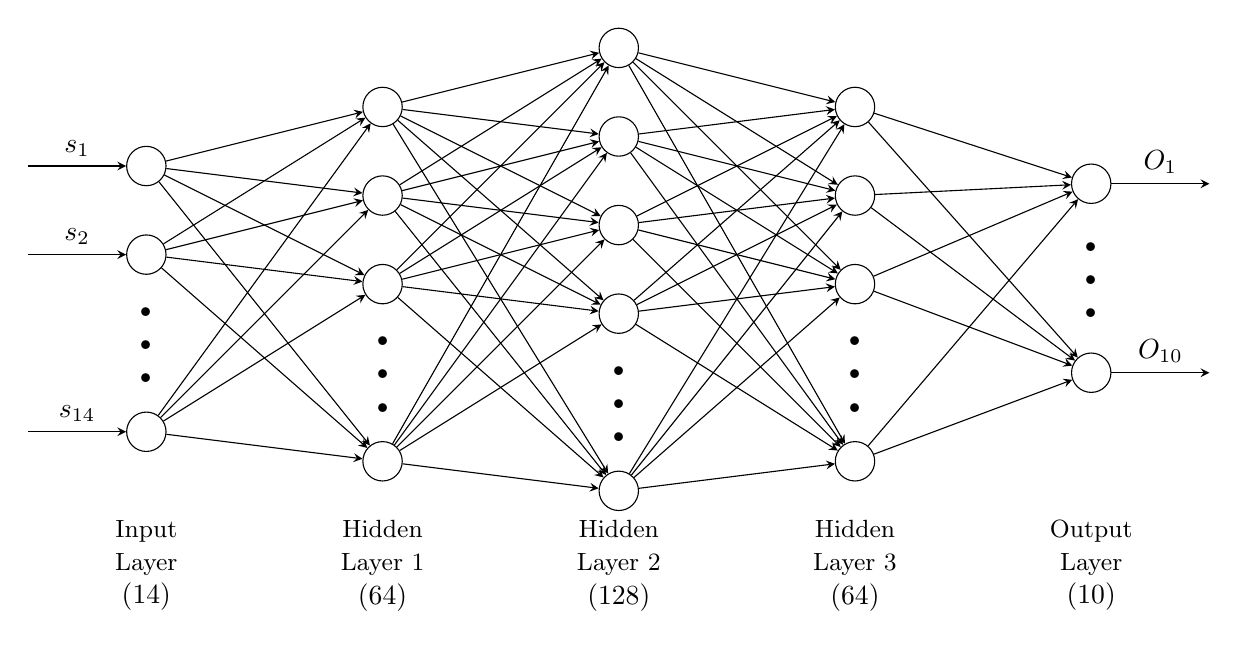
\begin{tikzpicture}[x=1.5cm, y=1.5cm, >=stealth, auto]
    
        \foreach \m/\l [count=\y] in {1,2,missing,3}
          \node [every neuron/.try, neuron \m/.try] (input-\m) at (0,2-\y*.75) {};
        \foreach \m [count=\y] in {1,2,3,missing,4}
          \node [every neuron/.try, neuron \m/.try ] (hidden1-\m) at (2,2.5-\y*0.75) {};
        \foreach \m [count=\y] in {1,2,3,4,missing,5}
          \node [every neuron/.try, neuron \m/.try ] (hidden2-\m) at (4,3-\y*0.75) {};
        \foreach \m [count=\y] in {1,2,3,missing,4}
          \node [every neuron/.try, neuron \m/.try ] (hidden3-\m) at (6,2.5-\y*.75) {};
        \foreach \m [count=\y] in {1,missing,2}
          \node [every neuron/.try, neuron \m/.try ] (output-\m) at (8,1.9-\y*.8) {};
        \foreach \l [count=\i] in {1,2,14}
          \draw [<-] (input-\i) -- ++(-1,0)
            node [above, midway] {$s_{\l}$};
        \foreach \l [count=\i] in {1,10}
          \draw [->] (output-\i) -- ++(1,0)
            node [above, midway] {$O_{\l}$};
        \foreach \i in {1,...,3}
          \foreach \j in {1,...,4}
            \draw [->] (input-\i) -- (hidden1-\j);
        \foreach \i in {1,...,4}
          \foreach \j in {1,...,5}
            \draw [->] (hidden1-\i) -- (hidden2-\j);
        \foreach \i in {1,...,5}
          \foreach \j in {1,...,4}
            \draw [->] (hidden2-\i) -- (hidden3-\j);
        \foreach \i in {1,...,4}
          \foreach \j in {1,...,2}
            \draw [->] (hidden3-\i) -- (output-\j);
        \foreach \l [count=\x from 0] in {\small Input \\\small Layer\\(14) ,\small Hidden \\\small Layer 1\\(64), \small Hidden \\\small Layer 2\\(128), \small Hidden \\\small Layer 3\\(64), \small Output \\\small Layer\\(10)}
          \node [align=center, below, yshift=-5.5cm] at (\x*2,2) {\l};
    \end{tikzpicture}
    \caption{DNN Architecture. This diagram depicts a DNN structure characterized by three hidden layers. The initial layer comprised the input data, also followed by a fully connected layer featuring 64 neurons. Subsequently, a second fully connected layer with 128 neurons establishes connections, followed by another fully connected layer with 64 neurons. It's worth highlighting that each of these fully connected layers is ignited by a Rectified Linear Unit (ReLU) function, which adds non-linearity to the network's computations. }
    \label{fig:NN}
\end{figure}
